\chapter{Simulação}
\label{chap:simulation}
Nessa seção, busca-se validar a abordagem integrada de Modelagem por meio de Redes de Petri Coloridas (RPC) e Controle Cooperativo. Para realizar essa validação, optou-se por empregar a estratégia de simulação, utilizando um sistema multiagente composto por diversos componentes, os quais foram concebidos para representar um ambiente similar a um sistema industrial.

Neste processo de simulação, são utilizadas ferramentas de software dedicadas à modelagem em RPC, com destaque para o CPN-Tools.\footnote{pode ser acessada em \texttt{https://cpntools.org/}} Essa ferramenta oferece funcionalidades específicas para a edição, simulação e análise de Redes de Petri Coloridas. A escolha do CPN-Tools visa proporcionar uma representação fiel e detalhada do sistema em estudo.

Para a implementação do algoritmo matemático de consenso, optou-se por utilizar a linguagem de programação Python. Essa escolha deve-se à reputação da linguagem como sendo de alto nível, funcional e orientada a objetos, oferecendo assim uma abordagem versátil e eficiente para a execução do algoritmo em questão.

Ao unir a simulação do sistema multiagente com as capacidades do CPN-Tools e a flexibilidade do Python, almeja-se obter resultados robustos que validem a eficácia da abordagem proposta. Esta seção detalhará o processo de simulação, desde a definição dos parâmetros até a análise crítica dos resultados obtidos, proporcionando uma compreensão clara e abrangente da validade e desempenho da abordagem integrada.

\section{Planta Industrial}
A gestão de vagões em uma planta industrial, que permite a ultrapassagem entre eles por meio de mudanças nas pistas, representa uma abordagem inovadora no contexto ferroviário industrial. Esse sistema dinâmico busca otimizar o movimento e a alocação de vagões, proporcionando flexibilidade e eficiência operacional.

Ao incorporar a capacidade de ultrapassagem, a planta industrial adquire versatilidade, possibilitando a reorganização estratégica dos vagões para atender a demandas específicas. Essa funcionalidade torna-se particularmente valiosa em situações onde é necessário priorizar determinados vagões, reduzir tempos de espera ou melhorar o desempenho global do sistema ferroviário dentro do contexto da planta industrial.

A implementação de mudanças nas pistas como um meio de permitir a ultrapassagem requer uma coordenação precisa e um controle eficaz do sistema. Técnicas como Redes de Petri Coloridas (RPC) ou algoritmos de controle cooperativo podem ser empregados para modelar e simular o comportamento dinâmico da planta, considerando as interações entre os vagões e as mudanças nas pistas.

Um exemplo de representação desse sistema escolhido é demonstrada na figura \ref{fig:pista_com_dois_agentes}, tal que:
\begin{itemize}
    \item Os componentes $L_1$ e $L_2$ ilustrados em formato triangular são os vagões que representam os dois autômatos, ou agentes do sistema.
    \item As curvas $d_1,d_2,..,d_6$ representam as pistas pelas quais os vagões se locomovem, de modo os dois vagões estão posicionados incialmente na pista denominada de $d_1$.
    \item os elementos $x_1,x_2,x_3,x_4$ representam as quatro chaves responsáveis por fazer a mudança de via, elas podem comutar em duas posições diferentes a posição $b$ que representa o caminho de menor comprimento ou a posição $a$ que representa o caminho de maior comprimento.
\end{itemize}

\begin{figure}[h]
\centering
\caption{Planta com pista, vagões e pontos de mudança de via }
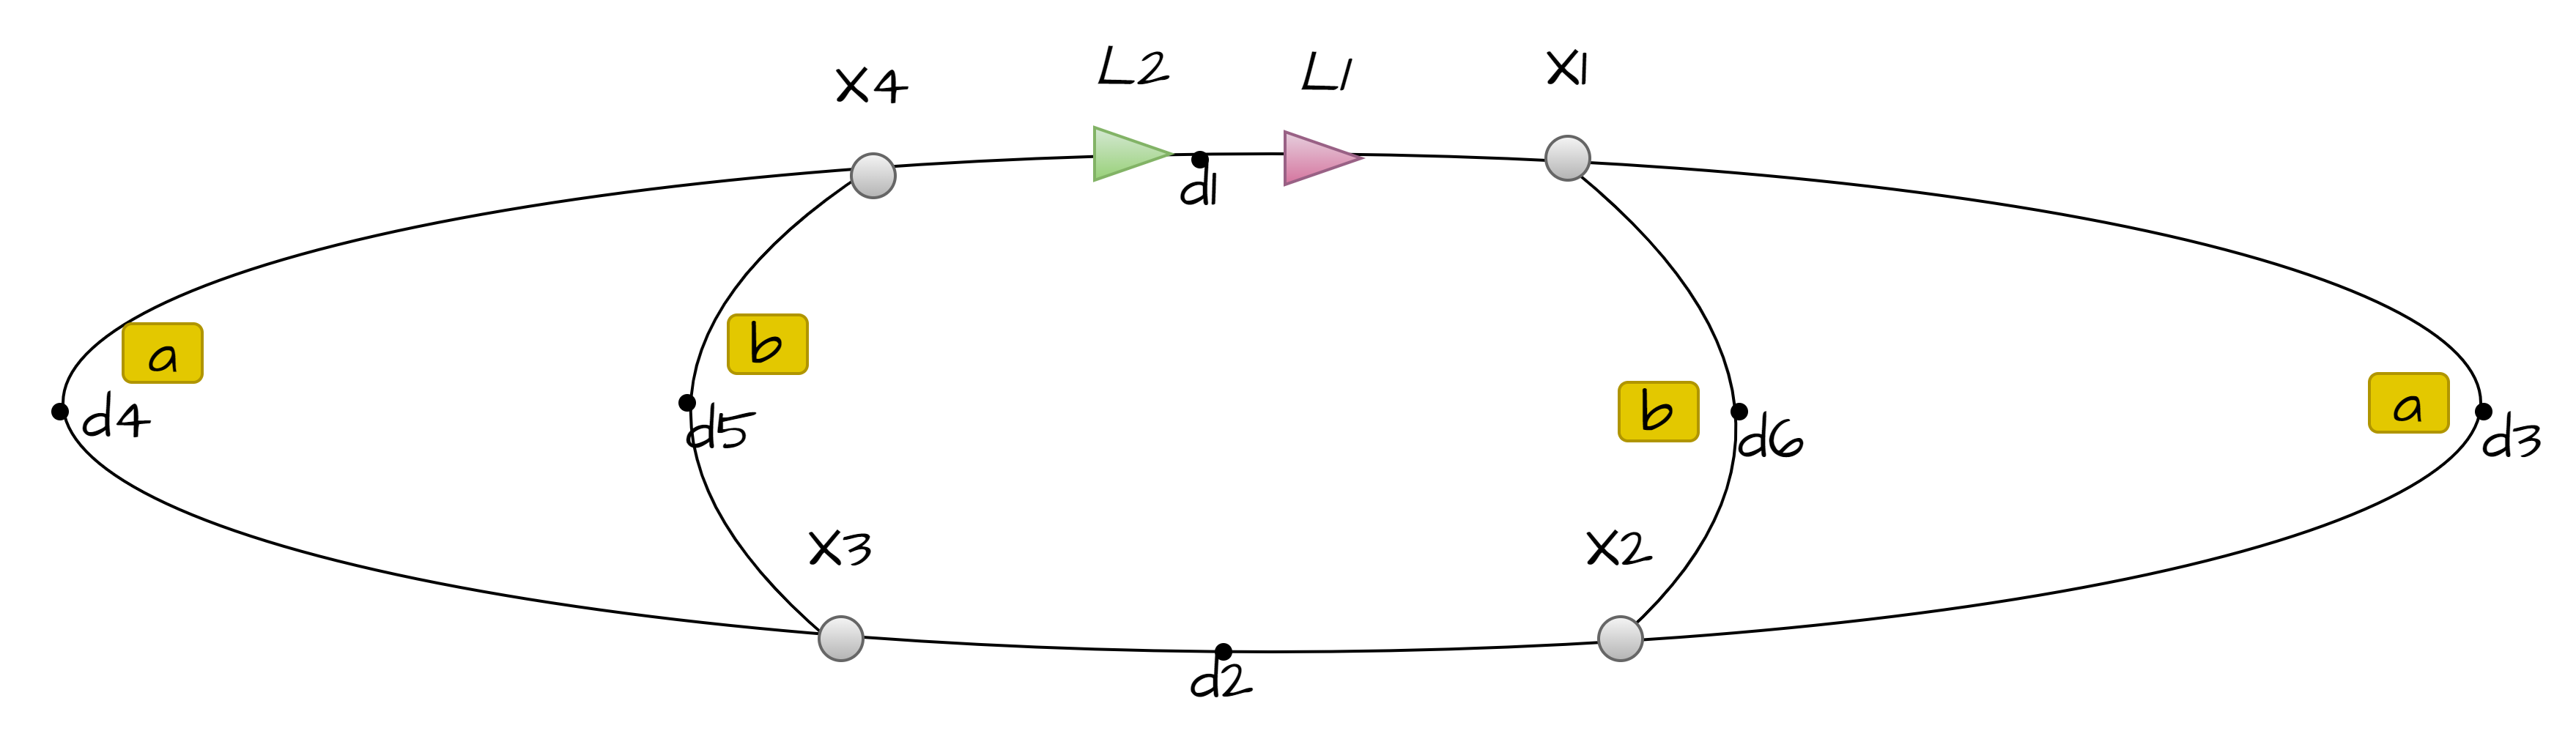
\includegraphics[width=1\linewidth]{figures/Simulation/Planta/planta_dois_agentes.png}
\label{fig:pista_com_dois_agentes}
\legend{Fonte: Elaborado pelo autor.}
\end{figure}

Para a simulação específica, os vagões movem-se entre pistas, e para efetuar uma ultrapassagem, é necessário que o vagão a ser ultrapassado siga pelo caminho mais longo, enquanto o vagão ultrapassante escolhe o caminho mais curto.

A chave de ultrapassagem foi designada como $x_1$. Quando o comando de ultrapassagem é acionado, inicialmente a chave se move para a posição $a$, assegurando o desvio para a pista mais longa. Em seguida, ela se move para a posição $b$, garantindo o desvio para a pista mais curta.

A chave $x_2$ desempenha o papel de primeiro desviar para a posição $b$, para receber o vagão da pista $d_6$. Posteriormente, comuta para a posição $a$, para receber o vagão da pista $d_3$.

As chaves $x_3$ e $x_4$ permanecem fixas na posição $b$, assegurando o percurso mais curto. Esse arranjo permite uma ultrapassagem de vagões de forma segura e otimizada entre as pistas.

\section{Modelagem Rede de Petri Colorida}
Para a modelagem do sistema proposto em Redes de Petri Colorida, foi definido o seguinte conjunto de cores para representar o tipo de token que vai ser alocado nos lugares da RPC de acordo com o seguinte quadro \ref{qua:conj_cores}.

\begin{quadro}[h]
\centering
\caption{Conjunto de Cores na RPC}
\begin{tabularx}{\textwidth}{|c|c|X|X|}
\hline
\textbf{Nomenclatura} & \textbf{Tipo}    & \textbf{Comando}                             & \textbf{Descrição} \\
\cline{1-4}
D & Inteiro & \texttt{colset D = int;} 
& Conjunto que indica a sequência dos vagões, onde o número 1 representa o vagão à frente, o número 2 representa o vagão atrás do 1, e assim por diante. \\ 
\cline{1-4}
X & String  & \texttt{colset X = string;} 
& Conjunto que representa a posição em que a chave se encontra, exemplo "a" para a posição A e "b" para a posição B. \\
\cline{1-4}
L & String  & \texttt{colset L = string;}         
& Conjunto de cores que representa os vagões ao longo da pista em que "L\_1" é o vagão L1 e "L\_2" o vagão L2. \\
\cline{1-4}
Ord & Record  & \texttt{colset Ord = record seq:D * train:L;} 
& Conjunto de cores que representa a associação do vagão L com a posição D,
de modo que caso "L1" esteja na primeira posição, será representado por "seq:1,train:L1". \\ 
\cline{1-4}

\end{tabularx}
\legend{Fonte: Elaborado pelo Autor}
\label{qua:conj_cores}
\end{quadro}

 Para cada conjunto de cores foi definido as variáveis correspondentes que serão alocados na inscrição dos arcos ao longo da RPC, de acordo com o quadro \ref{qua:variaveis_rpc}.

\begin{quadro}[ht]
\caption{Conjunto de Variáveis na RPC}
\begin{tabularx}{\textwidth}{|c|c|c|X|}
\cline{1-4}
% Cabeçalho
\textbf{Variável} & \textbf{Tipo} & \textbf{Exemplo} & \textbf{Descrição} \\ 
\cline{1-4} % Linha 1
d & D & 1`(1) ou 1`(2) & Variável de tipo Inteira, no exemplo tem-se 1 ficha com o valor 1, ou 2 fichas com valor 1, mais uma ficha com valor 2 \\ \cline{1-4} % Linha 2
x & X & 1`("a") ou 1`("b") & Variável do Tipo \textit{String} referente a posição de chave, pode ser do tipo "a" ou do tipo "b",como no exemplo. \\ \cline{1-4} % Linha 3
l & L & 1`("l1") ou 1`("l2") & Variável do Tipo \textit{String} referente ao vagão/trem que nos casos podem ser do tipo "l1" ou "l2", como no exemplo para dois agentes \\ \cline{1-4} % Linha 4
ord & Ord & 1`\{seq=2,train="l1"\} & Variável do Tipo \textit{record seq:d * train:L}, no exemplo descrito indica que o trem "l1" está na posição 2. \\ \cline{1-4} 
\end{tabularx}
\label{qua:variaveis_rpc}
\legend{Fonte:Elaborado pelo Autor}
\end{quadro}

Para a abstração e melhor organização e legibilidade da representação na RPC, foram definidos dois níveis hierárquico o nível mais acima da Pista, e o nível mais abaixo o de controle e comando. Cada nível possui um conjunto de módulos que podem ser agrupados em 3 principais funcionalidades, Pista, Controle das Chaves "X" e controle de Ordenação dos vagões "L", como demonstrado na figura \ref{fig:hierarquia_rpc}. Observa-se que para o controle das chaves X, foi definido 4 módulos de controle 1 para cada chave, que são responsáveis por gerenciar em qual posição cada respectiva chave irá estar. No caso do componente de Controle de Ordenação foram definidos 2 módulos, o de "Ordem", responsável por gerar o comando de "Ultrapassagem" ou "Não Ultrapassagem", já o módulo de "Inverter Ordem" é responsável por atualizar as ordem do vagões através da leitura da pista.

\begin{figure}[ht]
    \centering
    \caption{Modelo dos Componentes Hierárquicos da RPC}
    \label{fig:hierarquia_rpc}
    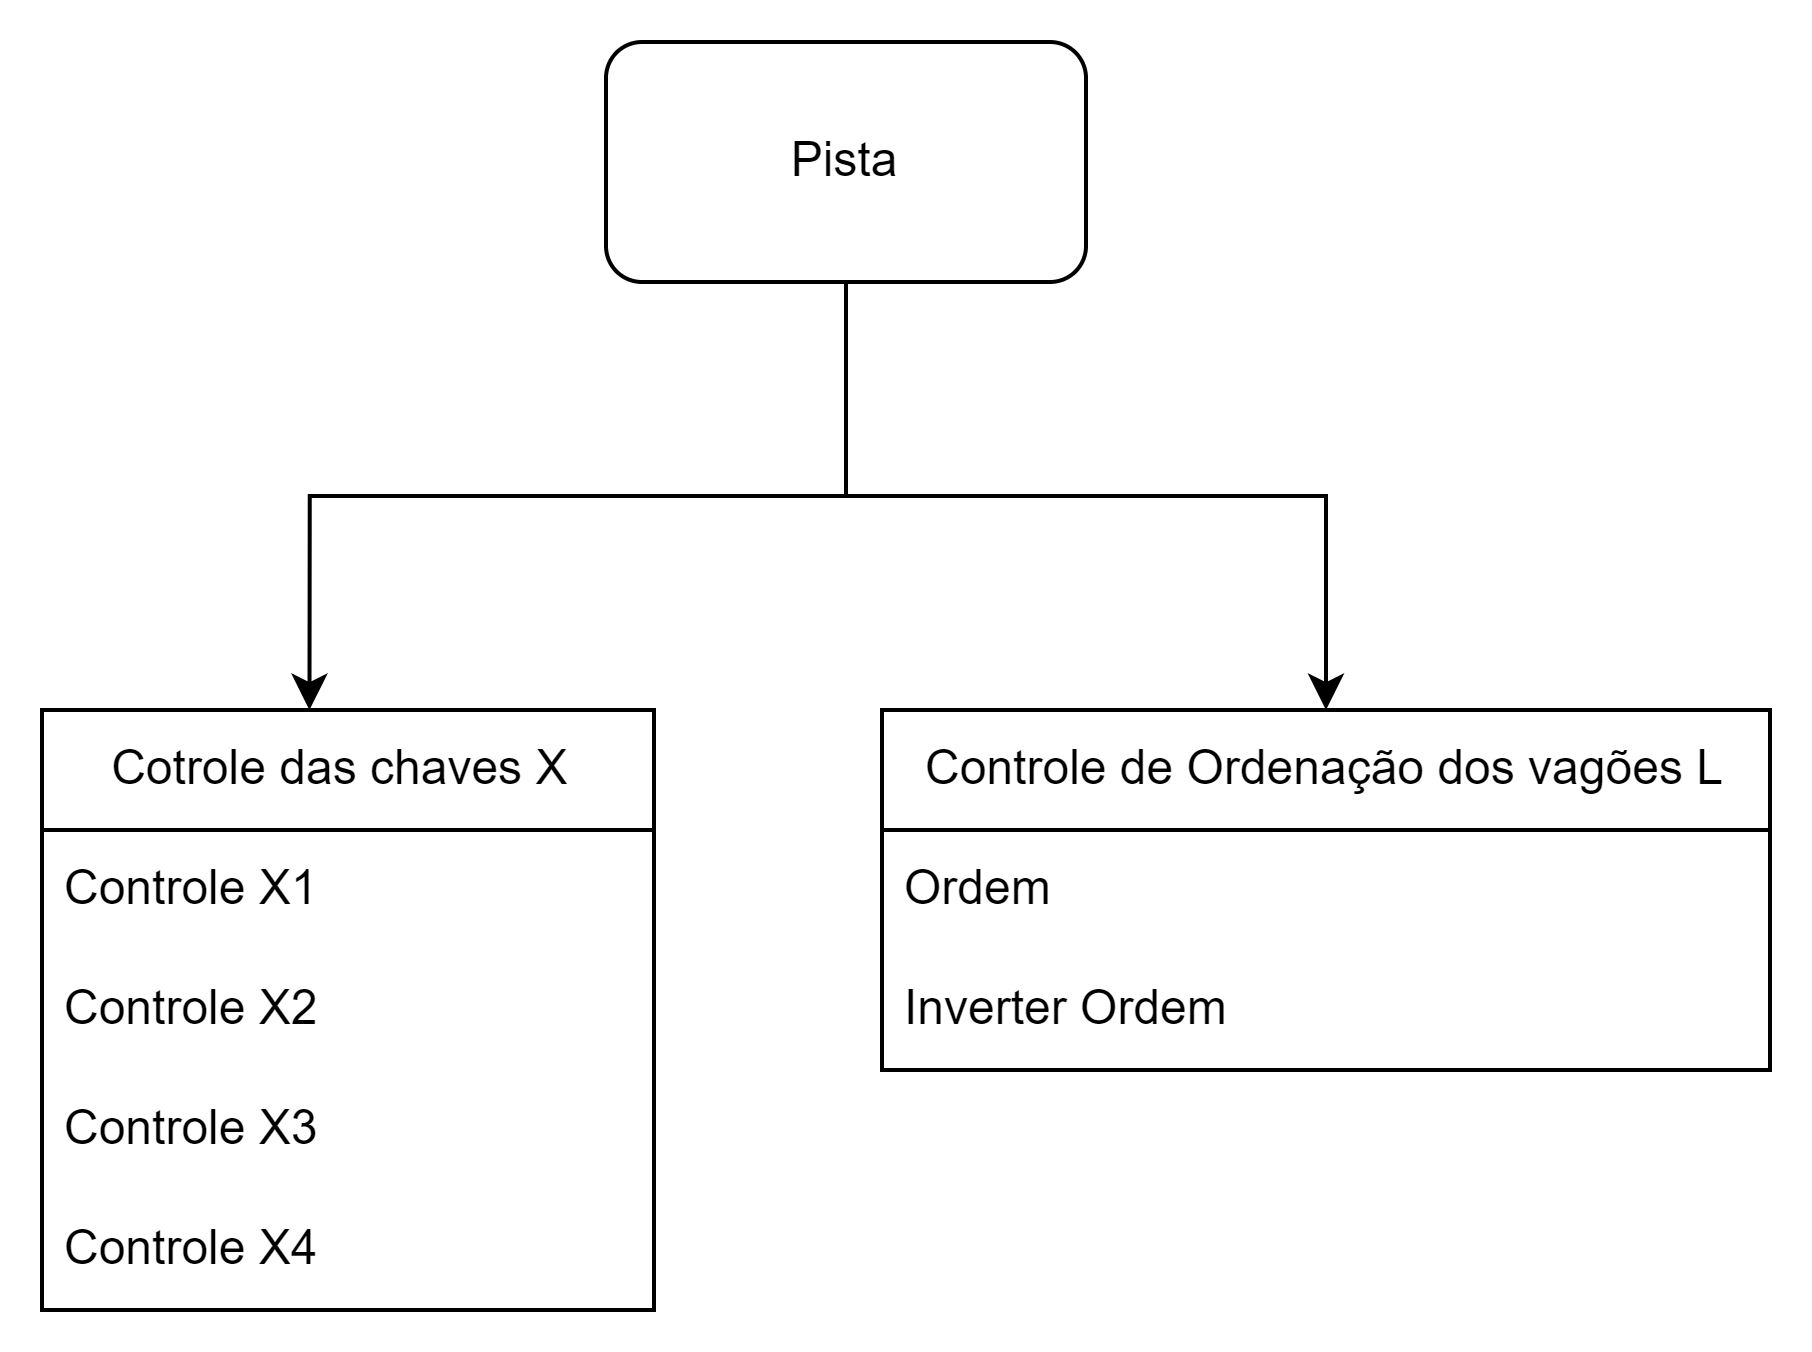
\includegraphics[width=0.8\linewidth]{figures//Simulation//Modelagem/hierarquia.png}
    \legend{Fonte: Próprio Autor}
\end{figure}

\subsection{Modelagem da Pista}
A modelagem da pista foi feito através do conjunto de lugares e transições que representam o movimento e mecanismos pelos quais os vagões iram transitar, a modelagem final da pista foi dividida em algumas mascaras (representação parcial da rede) para melhor visualização. 

A figura \ref{fig:pista_rpc} demonstra os principais componentes das pista, tal que os lugares de $d_1$ a $d_6$ referem-se as curvas da pista representada na figura \ref{fig:pista_com_dois_agentes}. Observe que o conjunto de cores nesses lugares são o conjunto $L$, indicando que neles transitam as fichas do tipo vagões que podem ser "$l_1$" ou "$l_2$" como nos casos do lugar $d_1\_p_1$ e $d_1\_p_2$ respectivamente. Assim de modo análogo os arcos que referentes a movimentação das fichas do tipo \textit{L} são da variável tipo \textit{l} que controla os graus de saída e entrada das transições que movimentam os vagões ao longo da pista. Também é modelado os locais de junções e divisões, por exemplo no lugar $d_1\_p_1$ que representa a área $1$ da pista $d_1$ nela a pista sofre uma divisão, de modo que o vagão pode ir ou para a curva $d_6$ ou para a curva $d_3$ da pista. Os locais de junção ocorrem por exemplo na curva $d_2\_p_1$ da pista, em que recebe tanto os vagões que veem da pista $d_3$, quanto da pista $d_6$.
\begin{figure}[ht]
    \centering
    \caption{Máscaras dos Componentes da pista na RPC}
    \label{fig:pista_rpc}
    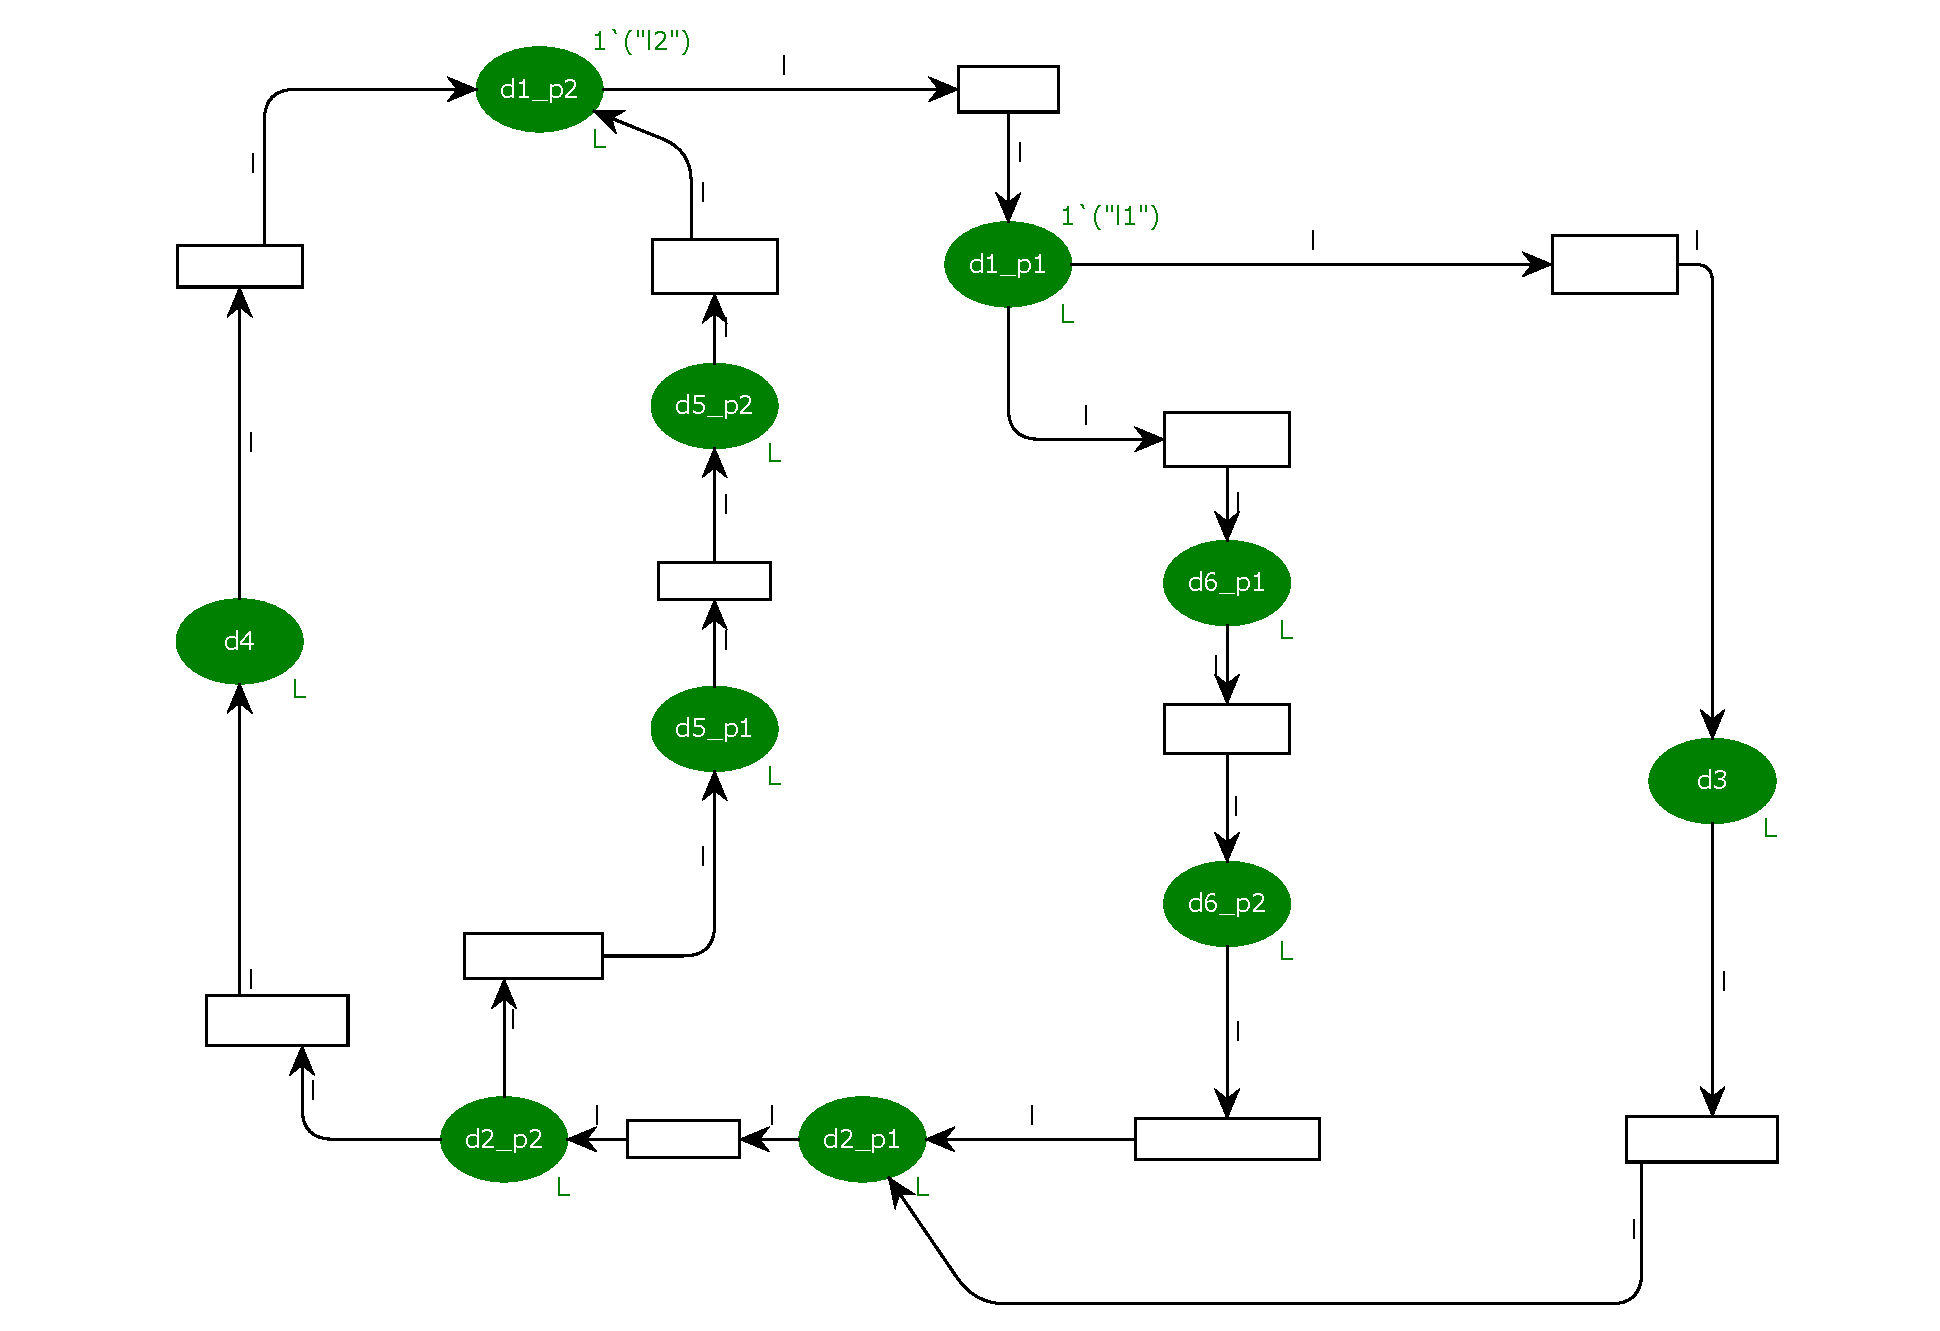
\includegraphics[width=1\linewidth]{figures//Simulation//Modelagem/pista.eps}
    \legend{Fonte: Próprio Autor}
\end{figure}
Considerando o modelo anterior de organização das pistas na figura \ref{fig:pista_chaves_rpc} representam além dos componentes fundamentas das curvas das pistas $d_1$ a $d_6$, os componentes de chaves \textit{X}, com as transições hierárquicas de \textit{Controle} $X_1$ a \textit{Controle} $X_4$. Observe que nos pontos de junção e divisão se encontroam os locais $X_1$ a $X_4$, que pertencem ao conjunto \textit{X} que podem receber fichas do tipo "a" ou "b" como explicado no quadro \ref{qua:variaveis_rpc}, tais lugares controlam as condições de acionamento das transições sd wusid d~so ligadas os arcos de saída. Por exemplo, 
\begin{figure}[ht]
    \centering
    \caption{Máscaras dos Componentes da pista com o controle das chaves na RPC}
    \label{fig:pista_chaves_rpc}
    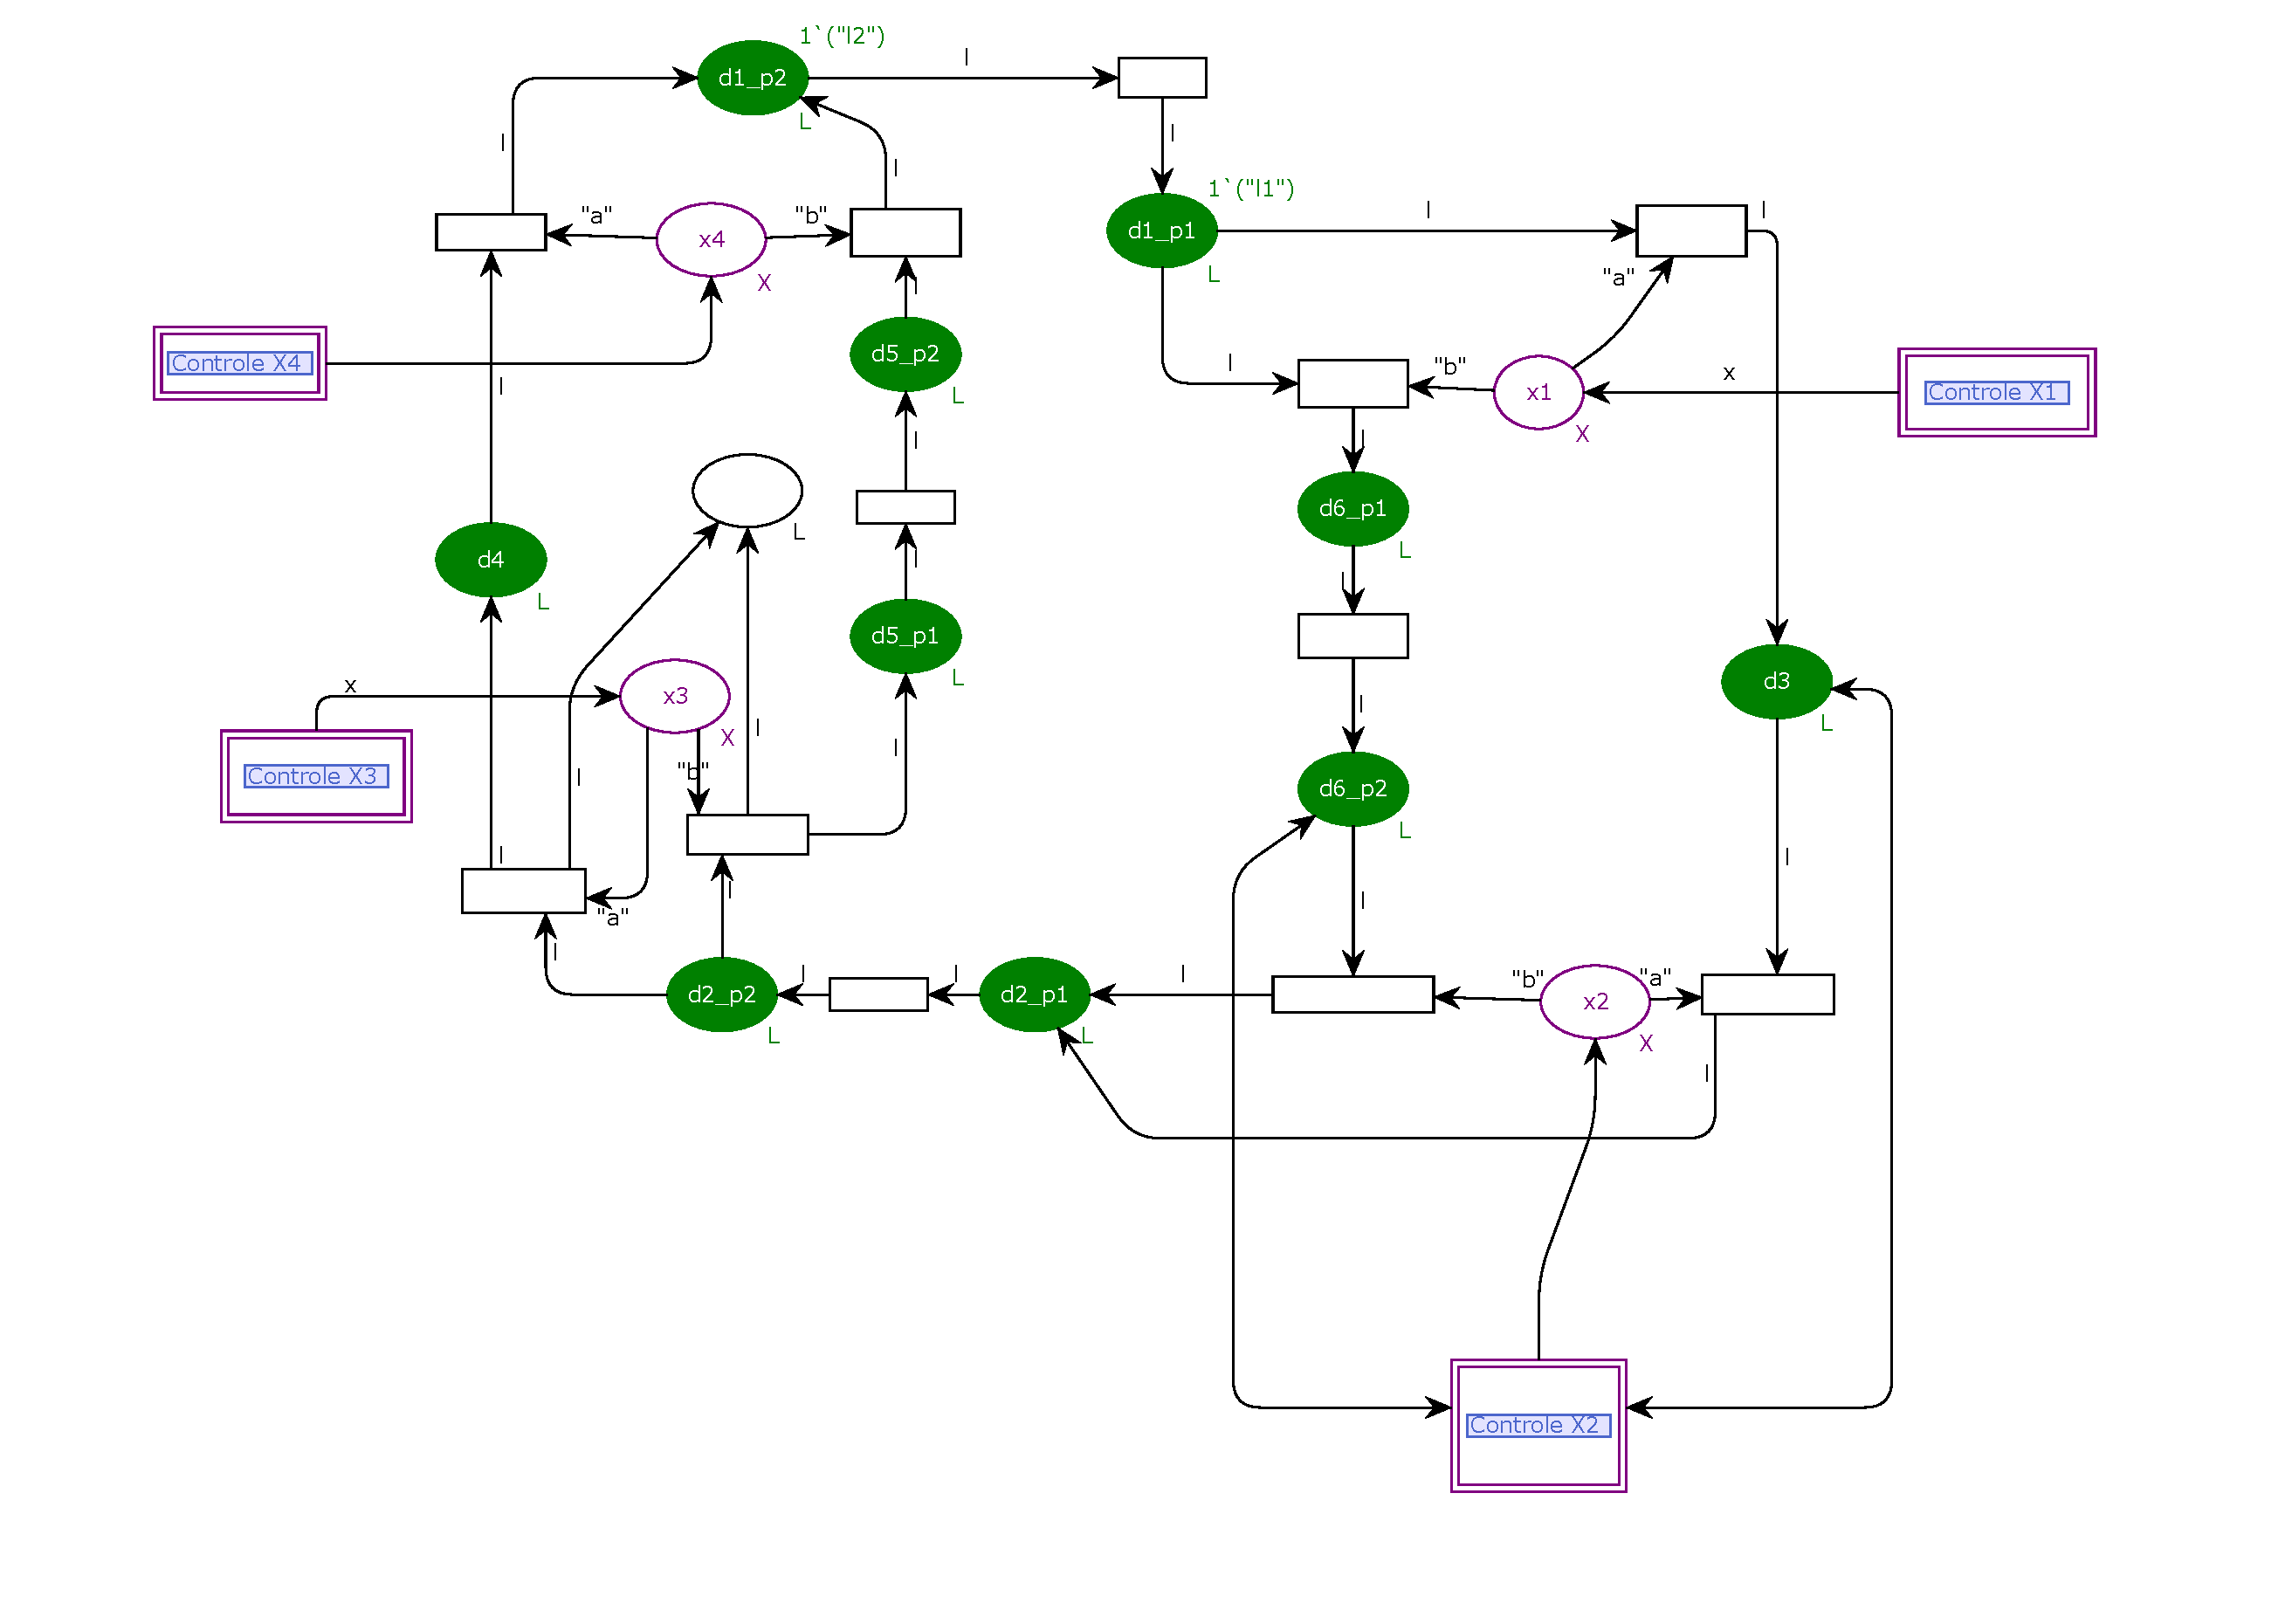
\includegraphics[width=1\linewidth]{figures//Simulation//Modelagem/pista_com_chaves.eps}
    \legend{Fonte: Próprio Autor}
\end{figure}
